\LARGE{ \textbf {Лекция №12}}\\
\Large{ \textbf {Алгоритм Лэнд и Дойг}}\\
Это алгоритмическая реализация метода ветвей и границ для решения задачи ЦЛП.\\
В этом алгоритме исходная целочисленная задача заменяется списком ее ослабленных линейных подзадач,
где условие целочисленности заменено на условие неотрицатеьности.
Подзадачи списка иерархически упорядоченны по своим допустимым решениям ,
это означает что области допустимых решений  подзадач являются подобластями области исходной задачи.
В соответсвии с общей схемой метода ветвей и границ список эти подзадач рекурсивно формируется  и расссматривается
в процедуре ветвления и оценке границ.

\textbf{Процедура ветвления }\\
Пусть на очередной итерации ис списка подзадач выбрана наиболее перспективная из подзадач,
однако не является целочисленным по одной переменной, $x_i$ - эту перменную можно выразить через отрицание свобоных переменных,
как принято в столбцовом Симплекс-методе.\\
$x_i = A_{i0} + \sum \limits_j A_{ij}-x_j^{i=0}$\\

Чтобы значение $x_i$ стало целым оно должно быть либо уменьшено до ближайшего целого снизу, либо увеличено до ближайшего целого сверху.
Можно подставить в эти дополнительные условия выражения для базисной переменной $x_i$.\\
Неравенство в левой подзадаче $x_i <= [A_{i0}]$\\
Неравенство в правой подзадаче $x_i => [A_{i0}] + 1$\\

В табличной форме, чтобы получить 2 новые подзадачи в списке нужно взять 2 копии оптимальной симплекс
таблицы выбранной перспективной от задачи списка, каждой копии нужно снизу добавить по одной строке для слабой переменной $y_i$
В левой подзадаче свободный член этой строки равен отрицанию дробной части свободного члена образующей строки,
а все коэффиценты равны отрицанию коэффицентов образующей строки $x_i$
В правой подзадаче свободный член дополнительной сроки равен дробной части свобоного члена образующей строки $x_i - 1$ ,
а все коэффиценты дополнительной строки равны кофэффицентам образующей строки.\\
\textbf{Процедура оценки границ.}\\
Это процедура должна осуществлять анализ перспективности подзадач списка.
 % - эта оценка определяется
\textit{При поиске максимума перспективной считается задача с максимальным оптимальным значением Z. При поиске минимума - минимальном.}
Для решения подзадач списка используется столбцовый алгоритм симплекс-метода, при этом начальная исходная ослабленная задача
может решаться либо прямым, либо двойственным симплекс-методом, в зависимомти от того является ли её опорный базис прямо или двойственнодопустимым.\\
А каждая из последующих задач решается столбцовым методом, при этом на первой симплексной итерации
за ведущую строку всегда выбирается дополнительная строка, для слабой переменной y.
Потому что это единственная отрицательная переменная в строке.\\
Процедуры ветвления и оценки границ чередуются на итерациях алгоритма.\\
А паралельно с решением задачи строится дерево решения. Его узлы - соответсвую подзадачм из списка,
ветви маркируются дополнительными условиями по дробной переменной и отражают иерархию подзадачт.
Решение должно продолжаться, пока не будет получена подзадача с оптимальным целочисленным решением,
которое является лучшим для подзадач в списке.

\textbf{Пример алгоритма.}\\

\begin{enumerate}
  \item ШАГ\\
  \begin{enumerate}
    \item Из строчки с целевой функцией выбирается столбец с наименьшии значением.
    \item В этом столбце находится такое число, что $ \frac{Z_0}{chislo} = min$. Это ведущая строка.
    \item Далее ведущий столбец делится на число из ведущей строки и записывается в следующую таблицу с обратным знаком.\\
    При этом столбец меняет имя на ведущую строчку.
    \item Затем к каждому столбцу прибавляется произведение его
    ведущего элемента(находящегося в ведущей строке в первой таблице) на ведущий столбец из новой таблицы.\\
    Получившуюся сумму записываем в новую таблицу.
  \end{enumerate}
  \item ШАГ\\
    \begin{enumerate}
      \item
    \end{enumerate}

\end{enumerate}

Найти максимальное значание функции цели \\
$z= x_1 + 2 x_2$\\
$2x_1 + 2x_2 <= 7$\\
$4x_1 - 5x_2 <= 9$\\
$x_1 , x_2 \in [0,1,2..]$\\

Canon\\
$z = x_1 + 2 x_2 $ \\
$2x_1 + 2x_2 + x_3^B = 7$\\
$4x_1 - 5x_2 + x_4^B = 9$\\

Dicanon\\
$z =  -(-x_1) -  2 (-x_2)$\\
$x_3 = 7 +2(-x_1)  + 2 (-x_2)$\\
$x_4 = 9 +4(-x_1)  + 5 (-x_2)$\\
\\
$ z_0 = 7 $\\
$x_1=0$\\
$x_2 =0  $\\

В ходе ветвления их значения не возрастают (оценок).\\
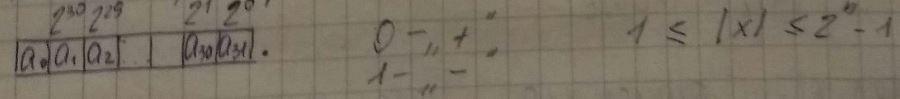
\includegraphics[width=\textwidth, height=\textheight]{3}
